\begin{figure}[h]
\centering
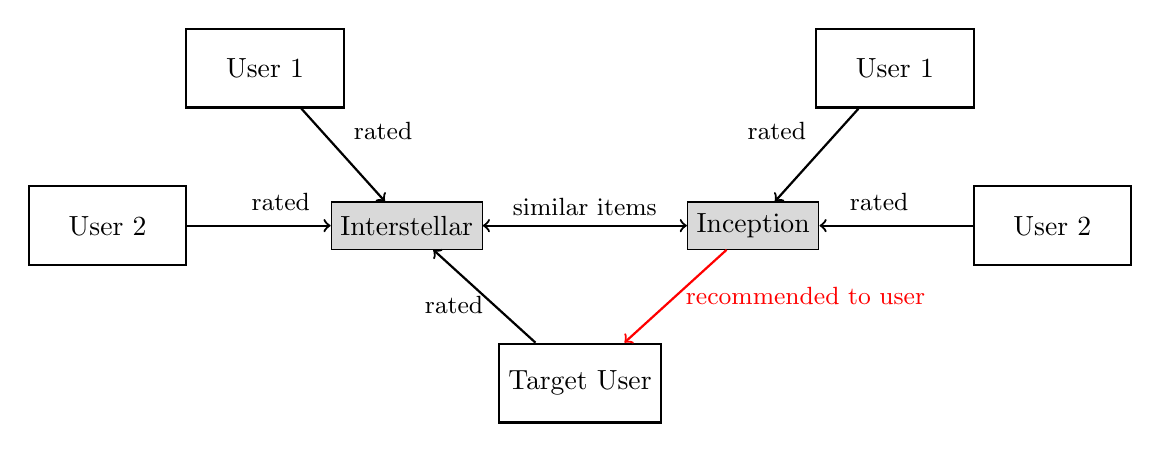
\begin{tikzpicture}[
    node distance=2cm,
    film/.style={circle, draw, minimum size=0.8cm, thick},
    user/.style={rectangle, draw, minimum width=2cm, minimum height=1cm, thick},
    movie/.style={rectangle, draw, minimum width=1.5cm, minimum height=0.6cm, fill=gray!30},
    arrow/.style={->, thick},
    redarrow/.style={->, thick, red},
    doublearrow/.style={<->, thick},
    label/.style={font=\small}
]

% Define positions
\coordinate (center) at (0,0);

% Target item and similar item
\node[movie] (similar_item) at (-2.2,0) {Interstellar};
\node[movie] (target_item) at (2.2,0) {Inception};

% Users for target item (left side)
\node[user] (user1) at (-4,2) {User 1};
\node[user] (user2) at (-6,0) {User 2};

% Users for similar item (right side)
\node[user] (user1b) at (4,2) {User 1};
\node[user] (user2b) at (6,0) {User 2};
\node[user] (target_user) at (0,-2) {Target User};

% Arrows from users to movies
\draw[arrow] (user1) -- (similar_item);
\node[label] at (-2.5, 1.2) {rated};

\draw[arrow] (user2) -- (similar_item);
\node[label] at (-3.8, 0.3) {rated};

\draw[arrow] (user1b) -- (target_item);
\node[label] at (2.5, 1.2) {rated};

\draw[arrow] (user2b) -- (target_item);
\node[label] at (3.8, 0.3) {rated};

\draw[arrow] (target_user) -- (similar_item);
\node[label] at (-1.6, -1) {rated};

% Similar items connection
\draw[doublearrow] (target_item) -- (similar_item) node[midway, above, label] {similar items};

% Recommendation arrow
\draw[redarrow] (target_item) -- (target_user) node[midway, right, label] {recommended to user};

\end{tikzpicture}
\caption{Item-based collaborative filtering. Similar items have similar ratings from the same users.}
\label{fig:item_based_collaborative_filtering}
\end{figure}